\section{Introduction}

This document details the deployment of Rubin IPsec tunnels between the summit network environment and the SLAC/Embargo network environment. It will also explain the physical and logical connections made to accomplish the integration with Rubin's summit network, to access the Long-Haul Network and provide an encrypted channel between both sites.


\subsection{Hardware}

As was explained on \href{https://ittn-043.lsst.io/}, the Rubin network is now using Arista Network as their main brand for routers and switches. As for the IPsec tunnels the hardware choosen was the Arista DCS-7280CR3MK-32D4S-R with an IPsec encryption module. 
To find the detailed datasheet please see \href{https://www.arista.com/assets/data/pdf/Datasheets/7280R3-Data-Sheet.pdf}

The Arista 7280R3 Series with encryption delivers high performance, large packet buffers, high scale and availability with wire speed
AES-256-GCM encryption. 

\begin{itemize}
\item 32 x QSFP100, 4 x QSFP-DD
\item CPU Quad-Core x86
\item System Memory 64GB
\item Packet Buffer Memory 8GB
\item 1U
\item Wire speed L2 and L3 forwarding
\item Up to 4.8Tbps of wire speed performance with 8GB of buffer
\item Broad connectivity with 25G SFP, 100G QSFP and 400G OSFP / QSFP-DD
\item Encryption Support for TunnelSec (QSFP100 Ports)
\end{itemize}

\begin{figure}
    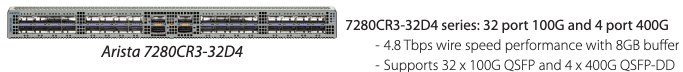
\includegraphics[width=9cm]{images/arista_datasheet01.png}
    \centering
    \caption{Arista DCS-7280CR3MK-32D4S}
  \end{figure}

There is a total of 4 Arista nodes, two of them are located in La Serena, Chile and the other two are at SLAC, US. 

\subsection{License}

Arista has an easy way to manage their licenses and for the IPsec switches there are 3 main licenses that are running at this moment, been the IPsec license the most important one.

Customer name:         Rubin Observatory
System Serial number:  JPA2322P328
System MAC address:    cc1a.a3dd.95e3
Domain name:           Unknown
Platform:              DCS-7280CR3MK-32D4S

License feature:  AHwSecSig 
        License parameter:  **info ommited** 
        Count:              1
        Start:              2023-10-11 00:00:00
        Expiration:         2123-09-17 00:00:00
        Active:             yes
        License source:     File


License feature:  IPSec 
        License parameter:  None
        Count:              4
        Start:              2023-10-11 00:00:00
        Expiration:         2123-09-17 00:00:00
        Active:             yes
        License source:     File


License feature:  MACsec 
        License parameter:  None
        Count:              4
        Start:              2023-10-11 00:00:00
        Expiration:         2123-09-17 00:00:00
        Active:             yes
        License source:     File


The licenses were activated on all four switches and will not expire until 2123.


\subsection{Support}

Arista provides a TAC support team reachable via email, phone or online channels. We now have a good understanding on how to engage with them and scalate our issues. We have been working very closely to solve the many problems we encountered during the deployment of this project.
The Arista TAC team has proved to be an useful asset during the deployment of the IPsec tunnels environment.  



